\documentclass{cpereport}
\usepackage{tikz}
\usepackage{amsmath}
\usepackage{amssymb}
\usepackage{hyperref}
\usepackage{pgfplots}

\begin{document}
\chapter{บทนำ}

\section{ความเป็นมาและความสําคัญของปัญหา}

แบบจำลองจักรกลเรียนรู้ (Machine Learning models) นั้นถูกใช้อย่างกว้างขวางในปัจจุบัน อย่างไรก็ตาม แบบจำลองใดๆ นั้นอาจมีความผิดพลาดต่อการทำการโจมตีประสงค์ร้าย (Adversarial attacks) เพื่อจงใจให้ผลลัพธ์ที่แบบจำลองนั้นคาดเดามีความผิดพลาดจากผลลัพธ์ที่ควรจะเป็น

ในการเรียนรู้เชิงตัวแปรเสริม (parameter-based learning) นั้น ตัวแปรเสริม (parameters) ค่าน้ำหนัก (weights) บนแบบจำลองการเรียนรู้เชิงลึก (deep Learning models) เป็นตัวกำหนดความฉลาดของแบบจำลอง อาจมีตัวแปรเสริมบางชุดที่ทำให้แบบจำลองมีช่องโหว่ต่อการโจมตีประสงค์ร้าย การโจมตีนั้นอาจเกิดจากการเพิ่มสัญญาณรบกวนซึ่งผ่านการคำนวน (calculated artefacts) เข้าสู่ข้อมูลรับเข้า (inputs) ซึ่งทำให้ความผิดพลาดของแบบจำลองในการพยากรณ์คำตอบนั้นเปลี่ยนไปอย่างชัดเจน 

โครงงานวิศวกรรมคอมพิวเตอร์นี้มุ่งหวังจะนำตัวแปรเสริมบนแบบจำลองมาสร้างภาพแสดง (visualise) ถึงจุดโหว่ในการพยากรณ์ใดๆ ของแบบจำลอง เพื่อลดความเสียหายอันอาจเกิดขึ้นได้จากการโจมตีแบบจำลองขณะถูกใช้งานจริง

\section{วัตถุประสงค์ของการศึกษา}
\noindent
โครงงานนี้มีวัตถุประสงค์และเป้าหมายดังนี้

\begin{enumerate}
    \item สร้างแบบจำลองเชิงลึก (Deep Learning models) ซึ่งสามารถถูกโจมตีประสงค์ร้าย (Adversarial attacks) ได้
    \item นำแบบจำลองในข้อ (1) มาสร้างเป็นรูปภาพแสดง (visualisation) เพื่อหาจุดโหว่ต่อการโจมตี รวมถึงคาดเดาแนวโน้มการโจมตีที่เป็นไปได้
    \item ใช้ความรู้ในข้อ (2) สร้างแบบจำลองที่ทนทาน (prone) ต่อการโจมตีมากขึ้น
\end{enumerate}

\section{ขอบเขตของการทําโครงงาน}
\noindent
โครงงานนี้มีขอบเขตการดำเนินงานดังนี้

\begin{enumerate}
    \item สร้างแบบจำลองเชิงลึก (Deep Learning models) ซึ่งสามารถถูกโจมตีประสงค์ร้าย (Adversarial attacks) ได้
    \item นำแบบจำลองในข้อ (1) มาสร้างเป็นรูปภาพแสดง (visualisation) เพื่อหาจุดโหว่ต่อการโจมตี รวมถึงคาดเดาแนวโน้มการโจมตีที่เป็นไปได้
    \item ใช้ความรู้ในข้อ (2) สร้างแบบจำลองที่ทนทาน (prone) ต่อการโจมตีมากขึ้น
\end{enumerate}

\section{ระยะเวลาและแผนดําเนินงาน}
ในช่วงแรกของการทำโครงงาน แผนการดำเนินงานนั้นจะใช้ในรูปแบบของรบวนทวนซ้ำ (iteration) ตามกรรมวิธีการดำเนินงานแบบเอไจล์ (agile) ซึ่งประกอบไปด้วยขั้นตอนการวนทวนดังนี้\dots

\section{ประโยชน์ที่คาดว่าจะได้รับ}
\begin{enumerate}
    \item เข้าใจถึงพื้นฐาน หลักการทำงาน และระบบจักรกลเรียนรู้แบบต่างๆ
    \item เข้าใจถึงจุดอ่อนของระบบจักรกลเรียนรู้ในแต่ละกรณี
    \item สามารถโจมตีระบบจักรกลเรียนรู้ เพื่อสร้างระบบจักรกลเรียนรู้ที่ทนทานต่อการโจมตีได้
\end{enumerate}

\section{คํานิยามศัพท์เฉพาะ}
\begin{itemize}
    \item \textbf{จักรกลเรียนรู้} (machine learning) คือระบบ หรือโค้ด หรือโปรแกรมคอมพิวเตอร์ที่เรียนรู้โครงสร้างของชุดคำถามและคำตอบโดยมิจำเป็นต้องทำการโปรแกรมลำดับการทำงานอย่างชัดแจ้ง (explicitly) 
    \item \textbf{การเรียนรู้เชิงโจมตี} (adversarial learning) หมายถึงการศึกษาถึงการโจมตีแบบจำลอง (model) ของจักรกลเรียนรู้ (machine learning)
\end{itemize}

\chapter{ทฤษฎีและงานวิจัยที่เกี่ยวข้อง}
\section{จักรกลเรียนรู้}
ระบบจักรกลเรียนรู้ (machine learning) อาจนิยามได้ว่าเป็นระบบที่ไม่ต้องมีการป้อนข้อมูล หรือวิธีทำงาน เข้าไปยังโค้ดโปรแกรมอย่างชัดแจ้ง (explicitly) โดยระบบดังกล่าวจะถูกฝึกสอนด้วยชุดของข้อมูลหรือประสบการณ์ (experience) และปรับตัวเองให้ส่งออกคำตอบซึ่งอิงจากประสบการณ์ที่ตนเองเคยได้เรียนรู้มา

หากจะกล่าวให้ละเอียด เราสามารถนิยามโปรแกรมซึ่งสามารถทำการ\textit{เรียน}ได้ดังนี้ \cite{Mitchell97}

\begin{definition}
โปรแกรมใดๆ เรียน (learn) จากประสบการณ์ (experience) $E$ บนงาน (task) $T$ และการวัดประสิทธิผล (performance measurement) $P$ หากประสิทธิผลบน $T$ ซึ่งถูกวัดโดย $P$ เพิ่มขึ้นตามประสบการณ์ $E$
\end{definition}

\section{การเรียนรู้เชิงลึก}
การเรียนรู้เชิงลึก (Deep Learning) คือความพยายามในการจำลองเซลล์ประสามของมนุษย์ให้อยู่ในรูปแบบจำลองคณิตศาสตร์
ด้วยความเชื่อทางหลักประสาทวิทยา (neurosciences) ว่าความฉลาดของสมองมนุษย์เกิดขึ้นได้จากโครงข่ายประสาทจำนวนมาก
ที่เชื่อมเข้าถึงกัน \cite{Goodfellow-et-al-2016}

\subsection{เปอร์เซปตรอน (Perceptron)}
\begin{figure}
    \centering
    \begin{tikzpicture}
        \def\layersep{2cm}
        \tikzstyle{neuron}=[circle,draw=black!100,minimum size=24pt, outer sep=3pt]
        \tikzstyle{annot}=[text width=5em, text centered]
        
        \node[neuron, pin=left:อคติ $b$] (bias) at (0, 0cm) {$w_0$};
        \foreach \name / \y in {1,...,3}
            \node[neuron, pin=left: ข้อมูลรับเข้า $x_\y$] (I-\name) at (0,-\y) {$w_\y$};
    
        \node[annot] (I-h) at (0, -4) {$\vdots$};
        \node[neuron, pin=left:ข้อมูลรับเข้า $x_n$] (I-4) at (0,-5) {$w_n$};

        \node[neuron] (sum) at (1*\layersep,-2 cm) {$\Sigma$};
        \node[neuron] (activation) at (3.75*\layersep,-2 cm) {$\sigma$};

        \foreach \source in {1,...,4}
            \draw [->] (I-\source) -- (sum);
        \draw [->] (bias) -- (sum);
        \draw [->] (sum) -- (activation) node [midway, above] (SumDesc) {$s = \left(\sum_{i=1}^{N} w_ix_i\right) + w_0$};
        \draw [->] (activation) -- (5.5*\layersep, -2cm) node [midway, above] (ActDesc) {ส่งออก $y = \sigma(s)$};
    \end{tikzpicture}
    \caption{เปอร์เซปตรอน}
    \label{tikz-perceptron}
\end{figure}
เปอร์เซปตรอน (Perceptron) \cite{rosenblatt_1958} เป็นแบบจำลองทางคณิตศาสตร์ของเซลล์สมองหนึ่งเซลล์ โดยมีคุณสมบัติดังนี้

\begin{itemize}
    \item รับเข้าข้อมูลมาในเซลล์จากหลายแหล่ง และให้น้ำหนักกับข้อมูลนั้นต่างกันไป
    \item ส่งออกข้อมูลเพียงค่าเดียว
\end{itemize}

ดังนั้น แบบจำลองทางคณิตศาสตร์สามารถเขียนออกมาจากหลักการสองข้อดังกล่าวได้ด้วยสมการ

$$ y = f\left(W^TX+b\right) $$

เมื่อ $W$ และ $X$ เป็นเมทริกซ์ขนาด $1 \times n$ (โดย $n$ เป็นจำนวนข้อมูลรับเข้า), $b$ เป็นค่าสัมประสิทธิ์คงที่ (อคติ: bias)
และ $f$ เป็นฟังก์ชั่นกระตุ้น (activation function) ซึ่งอาจเขียนรูปร่างของเปอร์เซปตรอนให้มีลักษณะรูปคล้ายเซลล์สมองได้ในลักษณะรูปที่ \ref{tikz-perceptron}

ยกตัวอย่างการใช้เปอร์เซปตรอนในการแก้ปัญหาอย่างง่ายได้ในที่นี้

\subsubsection{การคาดเดาราคาอสังหาริมทรัพย์}
หากสำรวจราคาอสังหาริมทรัพย์แล้วพบว่า
\begin{itemize}
    \item ราคาอสังหาริมทรัพย์จะเพิ่มขึ้นตามที่ดิน โดยเพิ่มขึ้นทุก 10,000 บาทต่อตารางวา
    \item ราคาอสังหาริมทรัพย์จะเพิ่มขึ้นตามจำนวนห้องนอน โดยเพิ่มขึ้นทุก 200,000 บาทต่อห้องนอน
    \item ราคาอสังหาริมทรัพย์จะลดลงตามจำนวนอายุปี โดยลดลงทุก 7,000 บาทต่ออายุของอสังหาริมทัพย์
    \item ราคากำหนดตรึง (fixed cost) ของอสังหาริมทรัพย์ อยู่ที่ 100,000 บาท
\end{itemize}
\noindent
จะสามารถเขียนเปอร์เซปตรอนเพื่อคาดเดาราคาอสังหาริมทรัพย์ได้โดย
$$ y = \sigma\left(W^TX\right) $$
เมื่อ $W$ ซึ่งเป็นค่าสัมประสิทธิ์แสดงถึงความสัมพันธ์ข้อมูลรับเข้า ซึ่งเขียนได้จากความสัมพันธ์ดังแสดงด้านล่าง
$$
    W^T = \begin{bmatrix}
        100000 & 10000 & 200000 & -7000
    \end{bmatrix}
$$
หากต้องการคาดเดาราคาบ้านที่มี 3 ห้องนอน เนื้อที่ 100 ตารางวา และมีอายุ 7 ปี จะสามารถเขียนเมทริกซ์ $X$ ได้เป็น
$$
    X = \begin{bmatrix}
        1 \\
        3 \\
        100 \\
        7
    \end{bmatrix}
$$
โปรดสังเกตว่า $x_0 = 1$ เนื่องจากผลคูณของเทอม $w_0$ และ $x_0$ เป็นค่าที่เรียกว่าค่าอคติ (bias) ของแบบจำลอง

เนื่องจากเปอร์เซปตรอนตัวนี้ถูกใช้ในการทำนายราคา ซึ่งกล่าวว่ามีความสัมพันธ์กันกับตัวแปรที่กำหนดข้างต้นในเชิงเส้น ดังนั้นจะกล่าวได้ว่าฟังก์ชั่นกระตุ้น (activation function) ที่เลือกใช้ จะเลือกใช้ฟังก์ชั่นเส้นตรง (linear function) $\sigma(x) = x$

ดังนั้น ผลการทำนายราคาบ้านคำนวนได้จาก
$$
    \begin{aligned}
        y &= \sigma\left(W^TX+b\right)\\
        &= \sigma\left(\begin{bmatrix}
            100000 & 10000 & 200000 & -7000
        \end{bmatrix} \times \begin{bmatrix}
            1 \\
            3 \\
            100 \\
            7
        \end{bmatrix}\right)\\
        &= \sigma(100000 + 30000 + 20000000 + (-49000)) = f(20981000)\\
        &= 20981000
    \end{aligned}
$$

\subsubsection{การสร้างประตูสัญญาณตรรกะด้วยเปอร์เซปตรอน}
เราสามารถสร้างประตูสัญญาณตรรกะ (logic gates) บางชนิดได้ด้วยเปอร์เซปตรอน เช่นการสร้าง AND และ OR gate

ยกตัวอย่างโครงสร้างของประตูสัญญาณและซึ่งสามารถสร้างได้ด้วยการกำหนดให้
\begin{itemize}
    \item $X$ เป็นเมทริกซ์ขนาด $1 \times 2$ กล่าวคือเมื่อรับค่า $x_1, x_2$ เป็นค่า 0 หรือ 1 แทนสัญญาณจริงหรือเท็จแล้ว
        $$X = \begin{bmatrix}
            1 \\
            a_1 \\
            a_2
        \end{bmatrix}$$
    \item กำหนดค่าของเมทริกซ์ $W$ เป็น
        $$W^T = \begin{bmatrix}
            -2 & 1 & 1
        \end{bmatrix}$$
    \item กำหนดฟังก์ชั่น $\sigma(x)$ เป็น step function กล่าวคือ
    $$
        \sigma(x) = \begin{cases}
            1; & x \geq 0\\
            0; & \textrm{ในกรณีอื่น}
        \end{cases}
    $$
\end{itemize}
และการสร้างประตูสัญญาณหรือสามารถทำได้ในลักษณะเดียวกันโดยเปลี่ยนชุดน้ำหนัก เป็น
        $$W^T = \begin{bmatrix}
            -1 & 1 & 1
        \end{bmatrix}$$

\subsection{เปอร์เซปตรอนแบบหลายชั้น (Multi Layer Perceptron)}

เราอาจสังเกตว่าเปอร์เซพตรอนหนึ่งตัวนั้นทำหน้าที่ได้เพียนแยก (classify) หรือถดถอย (regress) ปัญหาที่เป็นปัญหาเชิงเส้น (linear problems) ได้เท่านั้น อย่างไนก็ตามหากเรากำหนดให้ฟังก์ชั่น $f$ เป็นฟังก์ชั่นที่ไม่ใช่ฟังก์ชั่นเส้นตรงแล้ว เราอาจสร้าง\textbf{เปอร์เซปตรอนแบบหลายชั้น} (Multi Layer Perceptron) ขึ้นมาได้โดยมีลักษณะดังรูปที่ \ref{mlp}

\begin{figure}
    \centering
    \def\layersep{2.5cm}
    \begin{tikzpicture}[->,draw=black!70, node distance=\layersep]
        \tikzstyle{every pin edge}=[<-,shorten <=1pt]
        \tikzstyle{neuron}=[circle,draw=black!100,minimum size=17pt, outer sep=3pt]
        \tikzstyle{annot}=[text width=5em, text centered]
    
        \foreach \name / \y in {1,...,4}
            \node[neuron, pin=left:ข้อมูลรับเข้า \y] (I-\name) at (0,-\y) {};
    
        % Draw the hidden layer nodes
        \foreach \name / \y in {1,...,5}
            \path[yshift=0.5cm]
                node[neuron] (HA-\name) at (\layersep,-\y cm) {};
    
        \foreach \name / \y in {1,...,5}
            \path[yshift=0.5cm]
                node[neuron] (HB-\name) at (2*\layersep,-\y cm) {};

        \foreach \name / \y in {1,...,3}
            \path[yshift=-0.5cm]
                node[neuron] (O-\name) at (3*\layersep,-\y cm) {};
    
        \foreach \source in {1,...,4}
            \foreach \dest in {1,...,5}
                \path (I-\source) edge (HA-\dest);
    
        \foreach \source in {1,...,5}
            \foreach \dest in {1,...,5}
                \path (HA-\source) edge (HB-\dest);

        \foreach \source in {1,...,5}
            \foreach \dest in {1,...,3}
                \path (HB-\source) edge (O-\dest);

        \node[annot,above of=I-1, node distance=1cm] (hla) {ชั้นรับเข้า (ชั้นที่ 0)};
        \node[annot,above of=HA-1, node distance=1cm] (hla) {ชั้นซ่อน 1};
        \node[annot,above of=HB-1, node distance=1cm] (hla) {ชั้นซ่อน 2};
        \node[annot,above of=O-1, node distance=1cm] (hlb) {ชั้นส่งออก (ชั้นที่ 3)};
    \end{tikzpicture}
    \caption{เปอร์เซปตรอนแบบหลายชั้น}
    \label{mlp}
\end{figure}

เราอาจเขียนแทนน้ำหนักของโครงข่ายจากเปอร์เซปตรอนชั้นที่ $i$ ไปยังชั้นที่ $j$ ($j=i+1$) ได้เป็น
\begin{equation*}
    \boldsymbol{W}_{ij} = 
    \begin{bmatrix}
        w_{10} & w_{20} & \dots & w_{n_{i}0}\\
        w_{11} & w_{21} & \dots & w_{n_{i}1}\\
        w_{12} & w_{22} & \dots & w_{n_{i}2}\\
        \vdots & \vdots & \ddots & \vdots\\
        w_{1n_j} & w_{2n_j} & \dots & w_{n_jn_i}
    \end{bmatrix}
\end{equation*}
เมื่อจำนวนเปอร์เซปตรอนในชั้นที่ $k$ เขียนแทนด้วย $n_k$

ยกตัวอย่างเช่น เราจะสามารถสร้างประตูสัญญาณเฉพาะหรือ (XOR gate) ได้จากเปอร์เซปตรอนแบบหลายชั้นดังแสดงในรูปที่ \ref{xor-mlp} โดยเลขในแต่ละเปอร์เซปตรอนแทนค่าอคติ ($b$) และเลขบนเส้นเชื่อมแทนค่าน้ำหนัก ($w$) และกำหนดให้ฟังก์ชั่นกระตุ้น $\sigma$ เป็นฟังก์ชั่นขั้นบันได (step function) กล่าวคือ
\begin{equation*}
    \sigma(x) =
    \begin{cases}
        1; & x \geq 0\\
        0; & \textrm{ในกรณีอื่น}
    \end{cases}
\end{equation*}
เปอร์เซปตรอนดังกล่าว เมื่อรับค่า $A$ และ $B$ เป็น 0 หรือ 1 จะส่งออกค่า $A \oplus B$

\begin{figure}
    \def\layersep{2.5cm}
    \centering
    \begin{tikzpicture}[<-, draw=black!70, node distance=\layersep]
        \tikzstyle{edge}=[->,fill=white]
        \tikzstyle{neuron}=[circle,draw=black!100,minimum size=25pt, outer sep=3pt]
        \tikzstyle{annot}=[text width=5em, text centered]
    
        \node[neuron, pin=left:$A$] (I-1) at (0,0 cm) {$A$};
        \node[neuron, pin=left:$B$] (I-2) at (0,-2 cm) {$B$};
    
        \node[neuron] (HA-1) at (\layersep,-0 cm) {$-2$};
        \node[neuron] (HA-2) at (\layersep,-2 cm) {$-2$};

        \node[neuron] (O) at (2*\layersep,-1 cm) {$-1$};

        \path[edge]
            (I-1) edge node {$-1$} (HA-1)
            (I-1) edge node[very near end] {$1$} (HA-2)
            (I-2) edge node[very near end] {$1$} (HA-1)
            (I-2) edge node {$-1$} (HA-2)
            (HA-1) edge node {$1$} (O)
            (HA-2) edge node {$1$} (O)
        ;
    \end{tikzpicture}
    \caption{เปอร์เซปตรอนแบบหลายชั้นซึ่งทำหน้าที่เป็นประตูสัญญาณเฉพาะหรือ}
    \label{xor-mlp}
\end{figure}

\section{ฟังก์ชั่นกระตุ้นและความฉลาดของโครงข่ายประสาทเทียม}
\subsection{ทฤษฎีบทตัวประมาณฟังก์ชั่นครอบจักรวาล}
เหตุผลที่โครงข่ายประสาทเทียมสามารถทำงานได้ดี เนื่องจากมีการพิสูจน์ว่าโครงข่ายประสาทเทียมนั้นสามารถทำหน้าที่เป็นตัวประมาณฟังก์ชั่นครอบจักรวาล \cite{hornik_1991} (universal function approximator) กล่าวคือโครงข่ายประสาทเทียม $N: \mathbb{R} ^k \rightarrow \mathbb{R} ^n$ ที่มีความซับซ้อนมากเพียงพอ (ซึ่งจะกล่าวถึงความซับซ้อนนี้ในภายหลัง) สามารถที่จะจำลองฟังก์ชั่น $f: \mathbb{R}^k \rightarrow \mathbb{R}^n$ (กล่าวคือฟังก์ชั่นที่มีโดเมน และเรนจ์ เป็นจำนวนจริงใดๆ ในมิติที่เหมือนกับมิติข้อมูลรับเข้าและข้อมูลส่งออกของโครงข่ายประสาทเทียม $N$) ได้ \cite{Cybenko1989} \cite{Leshno1993} \cite{1910.03344}

บทพิสูจน์ของทฤษฎีนี้ทั้งในรูปแบบของกรณีไม่ตีกรอบความกว้าง (unbounded width case) และกรณีตีกรอบความกว้าง (bounded width case) สามารถศึกษาได้จากแหล่งอ้างอิง รวมถึงแหล่งอ้างอิงเพิ่มเติมที่ใช้การแสดงทัศนภาพ (visualisation) เพื่อการพิสูจน์ทฤษฎีบทดังกล่าว \cite{nielsen_1970}

\subsection{ข้อสังเกตต่อฟังก์ชันกระตุ้นและความฉลาด}

บทพิสูจน์ที่ได้กล่าวถึงไปก่อนหน้านี้สำหรับกรณีไม่ตีกรอบความกว้าง และตีกรอบความกว้าง เป็นบทพิสูจน์ที่ใช้ฟังก์ชันกระตุ้นเป็นฟังก์ชันซิกมอยด์ (sigmoid) และฟังก์ชันรีลู (ReLU) ตามลำดับ

อย่างไรก็ดี หากพิจารณาโครงข่ายประสาทเทียมใดๆ ที่ใช้ฟังก์ชันกระตุ้นเป็นฟังก์ชันเชิงเส้น $f(x) = x$ เราจะพบว่าโครงข่ายประสาทเทียมใดๆ จะสามารถยุบให้อยู่ในรูปของเปอร์เซปตรอนเพียงตัวเดียว และทำให้ไม่สามารถตัดสินใจปัญหาได้มากกว่าปัญหาที่แบ่งแยกเชิงเส้นได้ (linearly separable problems)

ดังนั้น อาจกล่าวด้วยการพิจารณา (intuition) ในลักษณะดังกล่าวได้ว่า ส่วนหนึ่งของความเป็นไปได้ของการที่โครงข่ายประสาทเทียมใดๆ สามารถทำหน้าที่เป็นตัวประมาณฟังก์ชันครอบจักรวาลได้ ส่วนหนึ่งมาจากการที่ฟังก์ชันกระตุ้นทำหน้าที่เป็นตัวบีบ (sqeezer) ช่วงของข้อมูลรับเข้าบนโดเมนจำนวนจริงใดๆ ($\mathbb{R}$) ให้กลายไปเป็นช่วงจำกัดช่วงอื่น (เช่นช่วง $(0, 1)$ ของฟังก์ชันซิกมอยด์ หรือช่วง $[0, \infty)$ ของฟังก์ชันรีลู)

\section{โครงข่ายประสาทเทียมแบบสังวัฒนาการ}

โครงข่ายประสาทเทียมแบบสังวัฒนาการ (Convolutional Neural Networks: CNN) \cite{lecun-1998} เป็นโครงข่ายประสาทเทียมซึ่งมักถูกใช้กับข้อมูลภาพ \cite{Krizhevsky-2012} โดยคร่าวแล้วโครงข่ายประสาทเทียมในลักษณะดังกล่าวมักประกอบด้วยชั้นประสาทเทียมในลักษณะดังนี้

\begin{itemize}
    \item \textbf{ชั้นสังวัฒนาการ} (convolution layer) เป็นชั้นที่กระทำตัวดำเนินการสังวัฒนาการ (convolve) ตัวกรอง (filter) $F$ บนข้อมูลนำเข้า $I$ ด้วยระยะเคลื่อน (stride) $S$ ผลลัพธ์จากการสังวัฒนาการนี้จะเรียกว่าแผนที่ลักษณะ (feature map) ยกตัวอย่างการสังวัฒนาการเพื่อหาเส้นเฉียงในรูปที่ \ref{conv-figure} สังเกตว่าการสังวัฒนาการด้วยตัวกรองเส้นเฉียงบนเส้นเฉียงบริเวณข้อมูลนำเข้า จะให้ค่าส่งออกที่มากกว่าการสังวัฒนาการตัวกรอกเส้นเฉียงบนจุดพื้นที่อื่นของข้อมูลนำเข้า (ในที่นี้เขียนแทนด้วยสีแดงเข้ม และสีแดงอ่อน)
    \item \textbf{ชั้นบ่อรวม} (pooling layer)
    เป็นชั้นที่ทำการสุ่มตัวอย่างแบบลดขนาด (downsampling) เพื่อลดขนาดของข้อมูลในขณะที่ยังคงไว้ซึ่งชุดคุณสมบัติที่ข้อมูลรับเข้ามี ชั้นบ่อรวมอาจแบ่งเป็นสองประเภทหลัก
    \begin{itemize} 
        \item \textbf{ชั้นบ่อรวมแบบมากสุด} (maximum pooling layer) เป็นชั้นบ่อรวมที่พบได้บ่อยที่สุด
        \item \textbf{ชั้นบ่อรวมแบบเฉลี่ย} (average pooling layer) เป็นชั้นบ่อรวมที่พบในโครงข่ายประสาทเทียมแบบสังวัฒนาการบางรูปแบบ เช่น LeNet
        \item \textbf{ชั้นเชื่อมต่อถึงกันหมด} (fully connected layer) ซึ่งมีลักษณะเหมือนเปอร์เซปตรอนแบบหลายชั้นทั่วไป
    \end{itemize}
\end{itemize}

\begin{figure}
    \centering
    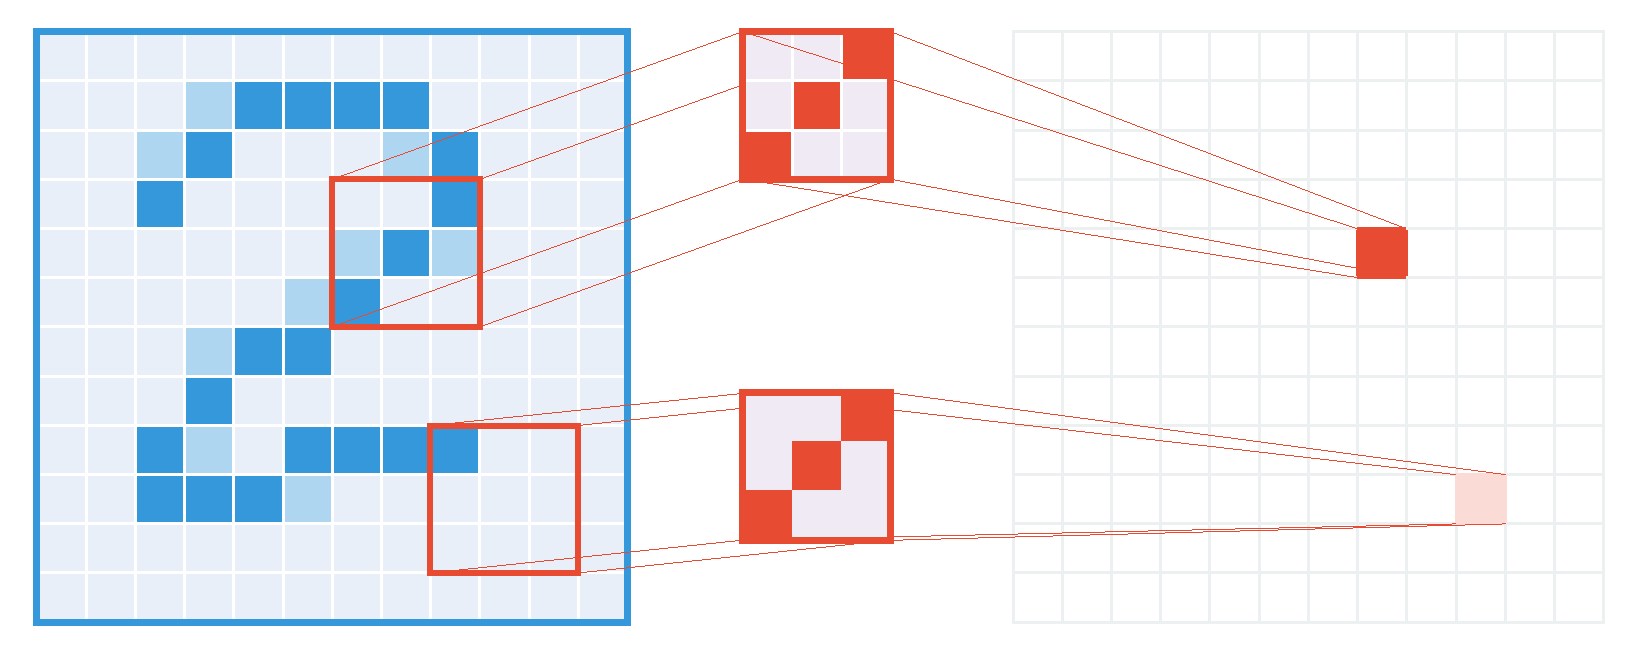
\includegraphics[width=0.8\textwidth]{images/convolution.pdf}
    \caption{ชั้นสังวัฒนาการ ซึ่งแสดงข้อมูลนำเข้าด้วยสีฟ้า และตัวกรองด้วยสีแดง}
    \label{conv-figure}
\end{figure}
\begin{figure}
    \centering
    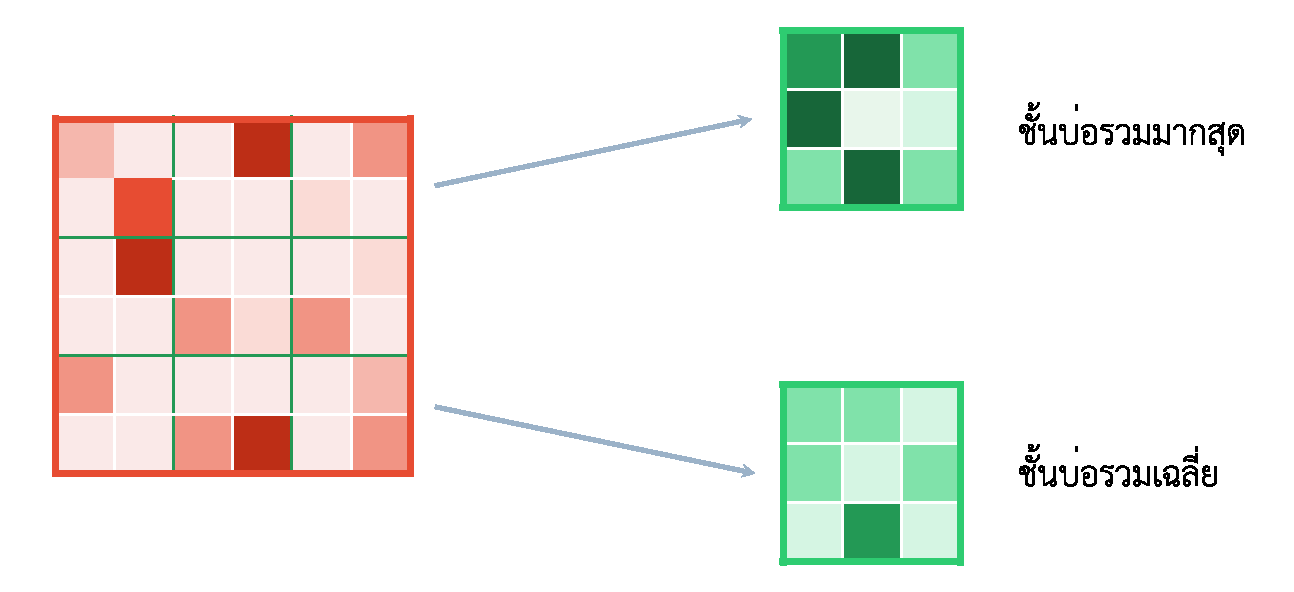
\includegraphics[width=0.8\textwidth]{images/pool.pdf}
    \caption{ชั้นบ่อรวม ทั้งแบบบ่อรวมมากสุดและแบบบ่อรวมเฉลี่ย โดยพิจารณาบ่อตามขอบเขตสีเขียว}
    \label{pool-figure}
\end{figure}
การสังวัฒนาการของชั้นสังวัฒนาการในโครงข่ายประสาทเทียม ทำหน้าที่เป็นตัวตรวจจับคุณสมบัติ (feature detector) เช่นการตรวจจับขอบ (edge detection) และชั้นบ่อรวมทำให้ขนาดของผลัพธ์จากชั้นสังวัฒนาการมีขนาดเล็กลง เพื่อให้จำนวนค่าน้ำหนักของโครงข่ายประสาทเทียมที่ต้องคำนวนนั้นน้อยลง

\section{การเรียนรู้ด้วยวิธีก้าวเคลื่อนถอยหลัง}

การเรียนรู้ด้วยวิธีก้าวเคลื่อนถอยหลัง (backpropagation learning) เป็นวิธีการเรียนรู้ที่ได้รับความนิยมมากที่สุดในปัจจุบัน ทั้งนี้ เราอาจพิจารณาการเรียนรู้ถอยหลังได้โดยทำความเข้าใจถึงฟังก์ชันสูญเสีย (loss function) และการปรับค่าตัวแปรเสริม (parameters) ดังนี้

\begin{figure}
    \centering
    \def\layersep{2.5cm}
    \begin{tikzpicture}[->,draw=black!70, node distance=\layersep]
        \tikzstyle{every pin edge}=[<-,shorten <=1pt]
        \tikzstyle{neuron}=[circle,draw=black!100,minimum size=17pt, outer sep=3pt]
        \tikzstyle{annot}=[text width=5em, text centered]
    
        \foreach \name / \y in {1,...,4}
            \node[neuron, pin=left:ข้อมูลรับเข้า \y] (I-\name) at (0,-\y) {};
    
        % Draw the hidden layer nodes
        \foreach \name / \y in {1,...,5}
            \path[yshift=0.5cm]
                node[neuron] (HA-\name) at (\layersep,-\y cm) {};
    
        \path[yshift=-1.5cm] node[neuron, fill=black!10] (O-1) at (2*\layersep,0 cm) {};
        \path[yshift=-1.5cm] node[neuron, fill=black!70] (O-2) at (2*\layersep,-1 cm) {};
        \path[yshift=-1.5cm] node[neuron, fill=black!20] (O-3) at (2*\layersep,-2 cm) {};
    
        \path[yshift=-1.5cm] node[neuron, fill=black!0] (T-1) at (3.5*\layersep,0 cm) {};
        \path[yshift=-1.5cm] node[neuron, fill=black!100] (T-2) at (3.5*\layersep,-1 cm) {};
        \path[yshift=-1.5cm] node[neuron, fill=black!00] (T-3) at (3.5*\layersep,-2 cm) {};

        \foreach \source in {1,...,4}
            \foreach \dest in {1,...,5}
                \path (I-\source) edge (HA-\dest);
    
        \foreach \source in {1,...,5}
            \foreach \dest in {1,...,3}
                \path (HA-\source) edge (O-\dest);

        \foreach \dest in {1,...,2}
            \path [<->] (T-\dest) edge (O-\dest);
        \draw [<->] (T-3) -- (O-3) node [midway, below] (losstext) {คำนวนค่าสูญเสีย};

        \node[annot,above of=I-1, node distance=1cm] (hla) {ชั้นรับเข้า};
        \node[annot,above of=HA-1, node distance=1cm] (hla) {ชั้นซ่อน};
        \node[annot,above of=O-1, node distance=1cm] (hlo) {ชั้นส่งออก};
        \node[annot,above of=T-1, node distance=1cm] (hlt) {คำตอบจริง};
    \end{tikzpicture}
    \caption{การคำนวนค่าสูญเสีย}
    \label{loss}
\end{figure}

\subsection{ค่าสูญเสีย}

ค่าสูญเสีย (loss) เป็นค่าที่ใช้ในการบอกว่าแบบจำลองใดๆ ตอบผิดมากหรือน้อยเพียงใด โดยค่าสูญเสียยิ่งมาก หมายถึงแบบจำลองตอบผิดมากเท่านั้น

ยกตัวอย่างเช่น หากเราสร้างแบบจำลองที่ต้องการส่งออกค่าเป็นค่าในลักษณะของการเข้ารหัสแบบหนึ่งจุดร้อน (one-hot encoding) ของค่าที่เป็นไปได้ 3 ชั้น (classes) จากข้อมูลตัวที่ i บนชุดฝึกหัด ดังแสดงในรูปที่ \ref{loss} ซึ่งต้องการคำตอบ $t_i$ ที่ถูกต้องเป็น
$$t_i = 
\begin{bmatrix}
    0 & 1 & 0
\end{bmatrix}
$$
ทว่า แบบจำลองกลับให้คำตอบ $o_i$ จากแบบจำลองเป็น
$$o_i = 
\begin{bmatrix}
    0.1 & 0.7 & 0.2
\end{bmatrix}
$$
เราอาจนิยามฟังก์ชันสูญเสียอย่างง่าย เพื่อยกตัวอย่างการคำนวนดังกล่าว โดยกำหนดให้ฟังก์ชันสูญเสียเป็นผลรวมของผลต่างกำลังสอง
$$
l_i\left(t_i, o_i\right) = \sum_{j=1}^{n}{\left(t_i[j] - o_i[j]\right)^2}
$$
ดังนั้น ในกรณีนี้ จะได้ค่าสูญเสียของจุดฝึกหัดนี้เป็น
\begin{align*}
    l_i\left(t_i, o_i\right) &= \sum_{j=1}^{n}{\left(t_i[j] - o_i[j]\right)^2}\\
    &= \left((0-0.1)^2 + (1-0.7)^2 + (0-0.2)^2\right)
\end{align*}
จะเห็นว่า ยิ่งค่า $t_i$ ใกล้เคียง $o_i$ มากขึ้นเท่าใด ค่าสูญเสียก็จะน้อยลงเท่านั้น

อย่างไรก็ตาม ฟังก์ชันสูญเสียในลักษณะดังกล่าว เป็นฟังก์ชันอย่างง่าย ในการฝึกสอนแบบจำลองทั่วไปมักนิยมใช้ฟังก์ชันอื่น เช่นค่าสูญเสียแบบความวุ่นวายข้ามชั้น (cross entropy loss) สำหรับการฝึกสอนแบบจำลองเพื่อการทำการจำแนกหมวดหมู่ (classification)
\bibliography{references/references} 
\bibliographystyle{ieeetr}
\end{document}